\documentclass[pdftex,a4paper]{scrreprt}
\usepackage[utf8]{inputenc}       
\usepackage[T1]{fontenc}
\usepackage{graphicx}
\usepackage{xcolor}
\usepackage{booktabs} % table rulers
\usepackage{longtable} % multipage tables


\usepackage[
	round,	%(defaultage in the main file and \input ) for round parentheses;
	authoryear,% (default) for author-year citations;
	sort,		% orders multiple citations into the sequence in which they 
]{natbib}	


\title{Supplemental Materials for the paper: \\Pesticides pollution of small streams in
Germany}
\author{Eduard Szöcs, Marvin Brinke, Bilgin Karaoglan, Ralf B. Schäfer}

\begin{document}
\maketitle

\listoffigures
\listoftables

\chapter{Data Cleaning}
Each of more then 30 datasets have been cleaned and homogenized separately, before combing in a common database.
Cleaning steps comprised (Figure~\ref{fig:data_cleaning} gives a graphical overview).

\begin{enumerate}
	\item Structure: Structure has been adjusted to the database structure.
	\item Coordinates: Coordinates have been transformed to a common Coordinate Reference System (DHDN / 3-Grad Gauss-Krüger Zone 3 (EPSG:31467) and duplicates merged.
	\item Chemicals: Chemical names and identifiers have been unified using the webchem package \citep{szocs_webchem:_2016}.
	\item  Identifiers: Unique identifiers have been assigned.
	\item Units: All concentrations have been converted to $\mu g/L$. Values below limit of quantification have be set to zero.
	\item Other meta-data: meta-data has been standardised.
	\item Temporal resolution: The temporal resolution of the database is 1 day. Date below this resolution has been aggregated by maximum.
	\item Validity Checks: Simple rules for validity checks have been implemented (e.g. no negative concentrations).
\end{enumerate}


\begin{figure}
	\centering
	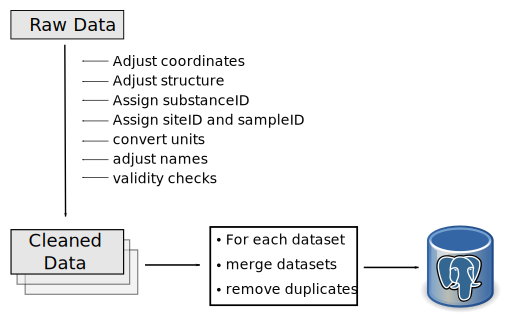
\includegraphics[width = 0.8\textwidth]{data_cleaning}
	\caption{Overview on data cleaning steps. After cleaning data has been stored in a relational spatial PostgreSQL database.}
	\label{fig:data_cleaning}
\end{figure}


\chapter{Overview on compiled data}
% Overview samples
% table generated in do_overview.R
\begin{table}[ht]
\centering
\caption[Overview on chemical samples.]{Overview on chemical samples. Only data from running waters and grab
sampling is shown. \textsuperscript{a}: Abbreviations according to ISO 3166-2:DE. 
      \textsuperscript{b}: Including metabolites} 
\label{tab:phch_overview}
\begin{tabular}{p{2.7cm}lllR{2cm}R{2cm}R{2cm}}
  \toprule
name & abbrv.\textsuperscript{a} & Begin & End & No. sites & No.samples & No. pesticides\textsuperscript{b} \\ 
  \midrule
Baden-Württemberg & BW & 2005-03-10 & 2014-10-02 & 7 & 172 & 98 \\ 
  Bavaria & BY & 2006-04-19 & 2013-12-17 & 13 & 218 & 155 \\ 
  Hesse & HE & 2007-01-15 & 2014-12-18 & 65 & 2411 & 144 \\ 
  Mecklenburg-Western Pomerania & MV & 2005-03-08 & 2014-12-17 & 130 & 1503 & 227 \\ 
  Lower Saxony & NI & 2014-03-24 & 2014-10-13 & 1 & 7 & 226 \\ 
  North Rhine-Westphalia & NW & 2005-01-18 & 2015-01-22 & 1139 & 8536 & 198 \\ 
  Rhineland-Palatinate & RP & 2008-01-02 & 2013-12-18 & 7 & 341 & 236 \\ 
  Schleswig-Holstein & SH & 2005-04-26 & 2014-11-26 & 269 & 1380 & 180 \\ 
  Saarland & SL & 2005-01-03 & 2013-11-25 & 2 & 104 & 57 \\ 
  Saxony & SN & 2005-01-02 & 2013-12-18 & 606 & 9141 & 173 \\ 
  Saxony-Anhalt & ST & 2005-01-24 & 2015-03-19 & 30 & 416 & 88 \\ 
  Thuringia & TH & 2005-06-16 & 2014-12-08 & 32 & 514 & 63 \\ 
   \midrule
 & Total & 2005-01-02 & 2015-03-19 & 2301 & 24743 & 478 \\ 
   \bottomrule
\end{tabular}
\end{table}



\begin{figure}
\centering
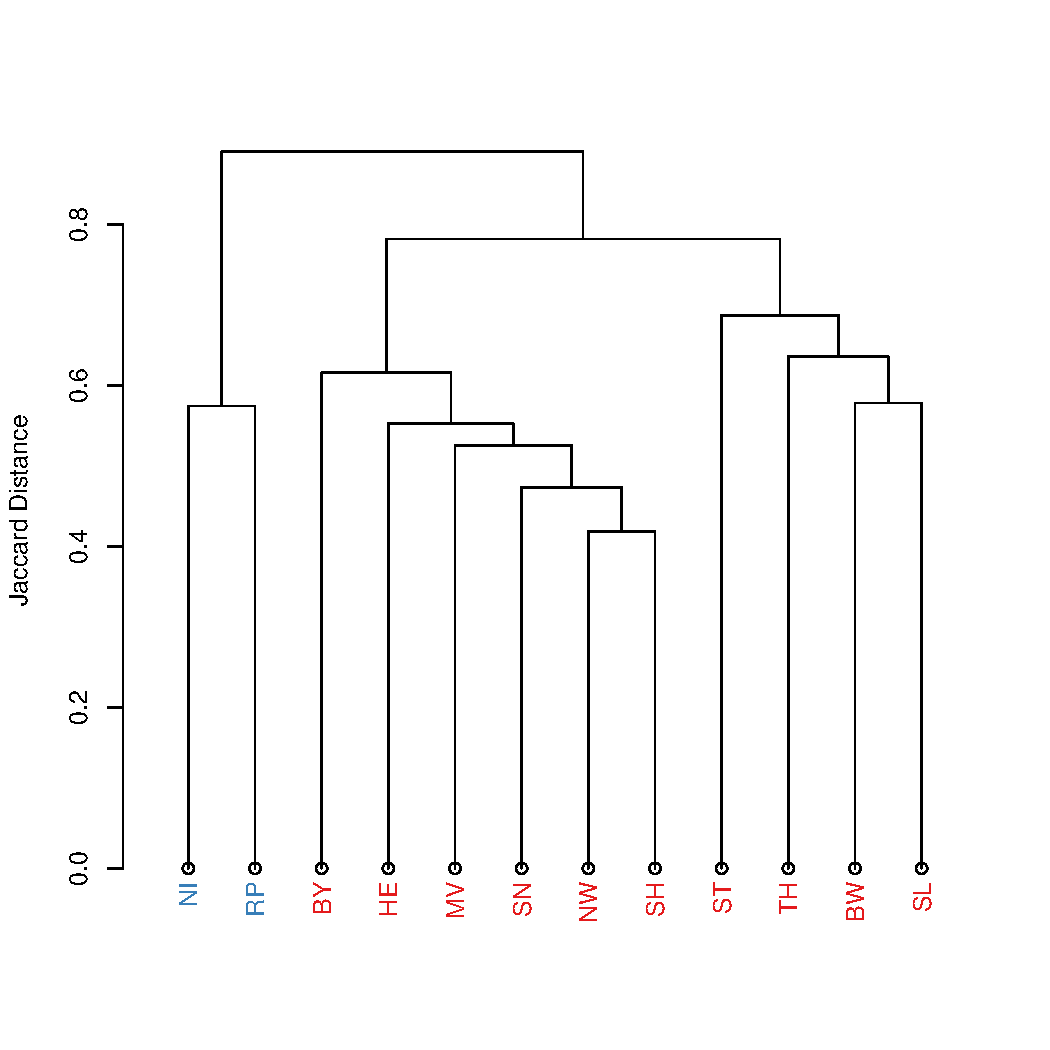
\includegraphics[width = 0.8\textwidth]{varclus}
\caption{Complete Linkage Cluster Dendrogram of Jaccard Similarity of analysed compound spectra between federal states. Abbreviations of state names according to ISO 3166-2:DE.}
\label{fig:varclus}
\end{figure}



% Overview variables
% table generated in do_overview.R
\begin{longtable}{lp{3cm}rlp{0.5cm}p{0.5cm}p{1cm}}
\caption[Overview on pesticides in the database.]{Overview on pesticides in the database. \
                    \textsuperscript{a} Authorized in Germany (Source: BVL, 2015). 
                    \textsuperscript{b} Authorized in the EU (Source: EU).
                    \textsuperscript{c} Regulatory Acceptable Concentration [ug/L] (Source: German EPA).} \\ 
  \toprule
 & Name & CAS & Group & Auth. GER\textsuperscript{a} & Auth. EU\textsuperscript{b} & RAC \textsuperscript{c} \\ 
  \midrule
1 & Bromoxynil & 1689-84-5 & herbicide & x & x & 3.30 \\ 
  2 & Ioxynil & 1689-83-4 & herbicide & x &  & 2.70 \\ 
  3 & Bentazon & 25057-89-0 & herbicide & x & x & 710.00 \\ 
  4 & Methoxychlor & 72-43-5 & insecticide &  &  &  \\ 
  5 & Thiometon & 640-15-3 & insecticide &  &  &  \\ 
  6 & Quintozen & 82-68-8 & fungicide &  &  &  \\ 
  7 & Vinclozolin & 50471-44-8 & fungicide &  &  &  \\ 
  8 & Pyrazophos & 13457-18-6 & fungicide &  &  &  \\ 
  9 & Quinalphos & 13593-03-8 & insecticide &  &  &  \\ 
  10 & Quinoxyfen (5,7-dichloro-4-(p-fluorophenoxy)quinoline) & 124495-18-7 & fungicide & x & x &  \\ 
  11 & 2,4-DB & 94-82-6 & herbicide &  & x &  \\ 
  12 & 2,4,5-T & 93-76-5 & herbicide &  &  &  \\ 
  13 & Alachlor & 15972-60-8 & herbicide &  &  &  \\ 
  14 & Ametryn & 834-12-8 & herbicide &  &  &  \\ 
  15 & Atrazin & 1912-24-9 & herbicide &  &  &  \\ 
  16 & Azinphos-ethyl & 2642-71-9 & insecticide &  &  &  \\ 
  17 & Bromacil & 314-40-9 & herbicide &  &  &  \\ 
  18 & Chlorfenvinphos & 470-90-6 & insecticide &  &  &  \\ 
  19 & Chloridazon & 1698-60-8 & herbicide & x & x & 56.00 \\ 
  20 & Chloroxuron & 1982-47-4 & herbicide &  &  &  \\ 
  21 & Chlorpyrifos & 2921-88-2 & insecticide &  & x & 0.00 \\ 
  22 & Chlortoluron & 15545-48-9 & herbicide & x & x & 2.30 \\ 
  23 & Cyanazin & 21725-46-2 & herbicide &  &  &  \\ 
  24 & Cypermetryn & 52315-07-8 & insecticide & x & x & 0.00 \\ 
  25 & Desethylatrazin & 6190-65-4 & metabolite &  &  &  \\ 
  26 & Desethylterbuthylazin & 30125-63-4 & metabolite &  &  &  \\ 
  27 & Desisopropylatrazin & 1007-28-9 & metabolite &  &  &  \\ 
  28 & Desmetryn & 1014-69-3 & herbicide &  &  &  \\ 
  29 & Diazinon & 333-41-5 & insecticide &  &  &  \\ 
  30 & Dichlorprop & 120-36-5 & herbicide &  &  &  \\ 
  31 & Dichlorvos & 62-73-7 & insecticide &  &  &  \\ 
  32 & Dicofol & 115-32-2 & insecticide &  &  &  \\ 
  33 & Diflufenican & 83164-33-4 & herbicide & x & x & 0.03 \\ 
  34 & Dimethoat & 60-51-5 & insecticide & x & x & 4.00 \\ 
  35 & Disulfoton & 298-04-4 & insecticide &  &  &  \\ 
  36 & Diuron & 330-54-1 & herbicide &  & x & 0.79 \\ 
  37 & Etrimfos & 38260-54-7 & insecticide &  &  &  \\ 
  38 & Fenitrothion & 122-14-5 & insecticide &  &  &  \\ 
  39 & Fenoprop & 93-72-1 & herbicide &  &  &  \\ 
  40 & Fenpropimorph & 67564-91-4 & fungicide & x & x & 0.20 \\ 
  41 & Fenthion & 55-38-9 & insecticide &  &  &  \\ 
  42 & Flurtamone & 96525-23-4 & herbicide & x & x & 0.99 \\ 
  43 & Hexazinon & 51235-04-2 & herbicide &  &  &  \\ 
  44 & Isoproturon & 34123-59-6 & herbicide & x & x & 1.30 \\ 
  45 & Linuron & 330-55-2 & herbicide &  & x &  \\ 
  46 & Malathion & 121-75-5 & insecticide &  & x &  \\ 
  47 & MCPA & 94-74-6 & herbicide & x & x & 9.00 \\ 
  48 & MCPB & 94-81-5 & herbicide &  & x &  \\ 
  49 & Mecoprop & 93-65-2 & herbicide &  & x & 160.00 \\ 
  50 & Metalaxyl & 57837-19-1 & fungicide &  & x & 46.00 \\ 
  51 & Metamitron & 41394-05-2 & herbicide & x & x & 38.00 \\ 
  52 & Metazachlor & 67129-08-2 & herbicide & x & x & 0.88 \\ 
  53 & Methabenzthiazuron & 18691-97-9 & herbicide &  &  &  \\ 
  54 & Methobromuron & 3060-89-7 & herbicide &  & x & 2.00 \\ 
  55 & Metolachlor & 51218-45-2 & herbicide &  &  &  \\ 
  56 & Metoxuron & 19937-59-8 & herbicide &  &  &  \\ 
  57 & Mevinphos & 7786-34-7 & insecticide &  &  &  \\ 
  58 & Monolinuron & 1746-81-2 & herbicide &  &  &  \\ 
  59 & Napropamid & 15299-99-7 & herbicide & x & x & 6.70 \\ 
  60 & Oxadixyl & 77732-09-3 & fungicide &  &  &  \\ 
  61 & Parathion-ethyl & 56-38-2 & insecticide &  &  &  \\ 
  62 & Parathion-methyl & 298-00-0 & insecticide &  &  &  \\ 
  63 & Penconazol & 66246-88-6 & fungicide & x & x & 3.20 \\ 
  64 & Pendimethalin & 40487-42-1 & herbicide & x & x & 0.63 \\ 
  65 & Pirimicarb & 23103-98-2 & insecticide & x & x & 0.09 \\ 
  66 & Prometryn & 7287-19-6 & herbicide &  &  &  \\ 
  67 & Propazin & 139-40-2 & herbicide &  &  &  \\ 
  68 & Propiconazol & 60207-90-1 & fungicide & x & x & 2.00 \\ 
  69 & Sebuthylazin & 7286-69-3 & herbicide &  &  &  \\ 
  70 & Simazin & 122-34-9 & herbicide &  &  &  \\ 
  71 & Tebuconazol & 107534-96-3 & fungicide & x & x & 0.58 \\ 
  72 & Terbutryn & 886-50-0 & herbicide &  &  &  \\ 
  73 & Terbuthylazin & 5915-41-3 & herbicide & x & x & 1.20 \\ 
  74 & Tolclofos-methyl & 57018-04-9 & fungicide & x & x &  \\ 
  75 & Triazophos & 24017-47-8 & insecticide &  &  & 0.03 \\ 
  76 & Trifluralin & 1582-09-8 & herbicide &  &  &  \\ 
  77 & Dicamba & 1918-00-9 & herbicide & x & x & 180.00 \\ 
  78 & Propetamphos & 31218-83-4 & insecticide &  &  &  \\ 
  79 & Aziprotryn & 4658-28-0 & herbicide &  &  &  \\ 
  80 & Norflurazon & 27314-13-2 & herbicide &  &  &  \\ 
  81 & Secbumeton & 26259-45-0 & herbicide &  &  &  \\ 
  82 & Tebutam & 35256-85-0 & herbicide &  &  &  \\ 
  83 & 2,4-D & 94-75-7 & herbicide & x & x & 1.10 \\ 
  84 & 4,6-Dinitro-o-Cresol & 534-52-1 & insecticide &  &  &  \\ 
  85 & Azinphos-methyl & 86-50-0 & insecticide &  &  &  \\ 
  86 & Azoxystrobin & 131860-33-8 & fungicide & x & x & 0.55 \\ 
  87 & Carbofuran & 1563-66-2 & insecticide &  &  &  \\ 
  88 & Epoxiconazol & 133855-98-8 & fungicide & x & x & 0.54 \\ 
  89 & Ethofumesat & 26225-79-6 & herbicide & x & x & 24.00 \\ 
  90 & Flufenacet & 142459-58-3 & herbicide & x & x & 2.40 \\ 
  91 & Lenacil & 2164-08-1 & herbicide & x & x & 0.65 \\ 
  92 & Metribuzin & 21087-64-9 & herbicide & x & x & 0.58 \\ 
  93 & Phenmedipham & 13684-63-4 & herbicide & x & x &  \\ 
  94 & Picolinafen & 137641-05-5 & herbicide & x & x & 0.04 \\ 
  95 & Propanil & 709-98-8 & herbicide &  &  &  \\ 
  96 & Dinoterb & 1420-07-1 & herbicide &  &  &  \\ 
  97 & Dinoseb & 88-85-7 & herbicide &  &  &  \\ 
  98 & Clodinafop & 114420-56-3 & herbicide & x & x &  \\ 
  99 & 2,6-Dichlorobenzamid & 2008-58-4 & metabolite &  &  &  \\ 
  100 & Aclonifen & 74070-46-5 & herbicide & x & x & 1.06 \\ 
  101 & AMPA & 1066-51-9 & metabolite &  &  &  \\ 
  102 & Atrazin, 2-Hydroxy & 2163-68-0 & metabolite &  &  &  \\ 
  103 & Benalaxyl & 71626-11-4 & fungicide & x & x & 20.00 \\ 
  104 & Bensulfuron-methyl & 83055-99-6 & herbicide &  & x &  \\ 
  105 & Bifenox & 42576-02-3 & herbicide & x & x &  \\ 
  106 & Boscalid & 188425-85-6 & fungicide & x & x & 12.50 \\ 
  107 & Carbendazim & 10605-21-7 & fungicide &  &  & 0.15 \\ 
  108 & Clomazon & 81777-89-1 & herbicide & x & x & 5.70 \\ 
  109 & Clopyralid & 1702-17-6 & herbicide & x & x & 1080.00 \\ 
  110 & Clothianidin & 210880-92-5 & insecticide & x & x & 0.01 \\ 
  111 & Cyprodinil & 121552-61-2 & fungicide & x & x & 0.75 \\ 
  112 & Dimefuron & 34205-21-5 & herbicide &  &  & 0.83 \\ 
  113 & Dimethachlor & 50563-36-5 & herbicide & x & x & 3.50 \\ 
  114 & Endosulfan, alpha & 959-98-8 & insecticide &  &  &  \\ 
  115 & Endosulfan, beta & 33213-65-9 & insecticide &  &  &  \\ 
  116 & Fenhexamid & 126833-17-8 & fungicide & x & x & 10.10 \\ 
  117 & Fenpropidin & 67306-00-7 & fungicide & x & x &  \\ 
  118 & Fenuron & 101-42-8 & herbicide &  &  &  \\ 
  119 & Fluopicolide & 239110-15-7 & fungicide & x & x &  \\ 
  120 & Fluroxypyr & 69377-81-7 & herbicide & x & x & 16.00 \\ 
  121 & Flusilazol & 85509-19-9 & fungicide &  &  & 1.10 \\ 
  122 & Glufosinat & 51276-47-2 & herbicide & x & x &  \\ 
  123 & Glyphosate & 1071-83-6 & herbicide & x & x & 100.00 \\ 
  124 & Haloxyfop & 69806-34-4 & herbicide &  &  &  \\ 
  125 & HCH, gamma (Lindan) & 58-89-9 & insecticide &  &  &  \\ 
  126 & Imidacloprid & 138261-41-3 & insecticide & x & x & 0.01 \\ 
  127 & Kresoxim-methyl & 143390-89-0 & fungicide & x & x & 1.00 \\ 
  128 & Metolachlorsäure & 152019-73-3 & metabolite &  &  &  \\ 
  129 & Metolachlorsulfonsäure & 171118-09-5 & metabolite &  &  &  \\ 
  130 & Nicosulfuron & 111991-09-4 & herbicide & x & x & 0.09 \\ 
  131 & Picoxystrobin & 117428-22-5 & fungicide & x & x & 0.60 \\ 
  132 & Prochloraz & 67747-09-5 & fungicide & x & x & 5.00 \\ 
  133 & Prosulfocarb & 52888-80-9 & herbicide & x & x & 3.80 \\ 
  134 & Quinmerac & 90717-03-6 & herbicide & x & x & 316.00 \\ 
  135 & Triadimenol & 55219-65-3 & fungicide & x & x & 3.40 \\ 
  136 & Fluazifop & 69335-91-7 & herbicide &  &  &  \\ 
  137 & Fenoxaprop & 95617-09-7 & herbicide &  &  &  \\ 
  138 & Esfenvalerat & 66230-04-4 & insecticide & x & x &  \\ 
  139 & Cyhalothrin (Summe Isomere) & 91465-08-6 & insecticide & x & x &  \\ 
  140 & Cyfluthrin (Summe Isomere) & 68359-37-5 & insecticide &  &  &  \\ 
  141 & Acifluorfen & 50594-66-6 & herbicide &  &  &  \\ 
  142 & Diclofop & 40843-25-2 & herbicide &  & x &  \\ 
  143 & Flamprop & 58667-63-3 & herbicide &  &  &  \\ 
  144 & Diflubenzuron & 35367-38-5 & insecticide &  & x &  \\ 
  145 & Difenoconazol & 119446-68-3 & fungicide & x & x & 0.36 \\ 
  146 & Amidosulfuron & 120923-37-7 & herbicide & x & x &  \\ 
  147 & Triasulfuron & 82097-50-5 & herbicide & x & x &  \\ 
  148 & Triflusulfuron & 135990-29-3 & herbicide & x & x &  \\ 
  149 & Methidathion & 950-37-8 & insecticide &  &  &  \\ 
  150 & Cyproconazol & 94361-06-5 & fungicide & x & x &  \\ 
  151 & Ethidimuron & 30043-49-3 & herbicide &  &  &  \\ 
  152 & Monuron & 150-68-5 & herbicide &  &  &  \\ 
  153 & Carbetamid & 16118-49-3 & herbicide &  & x &  \\ 
  154 & Triallat & 2303-17-5 & herbicide &  & x &  \\ 
  155 & Dichlobenil & 1194-65-6 & herbicide &  &  &  \\ 
  156 & Endosulfansulfat & 1031-07-8 & metabolite &  &  &  \\ 
  157 & Flurochloridon & 61213-25-0 & herbicide &  & x &  \\ 
  158 & Triclopyr & 55335-06-3 & herbicide & x & x &  \\ 
  159 & Fenoxycarb & 72490-01-8 & insecticide &  & x &  \\ 
  160 & Desmedipham & 13684-56-5 & herbicide & x & x &  \\ 
  161 & Flumioxazin & 103361-09-7 & herbicide & x & x &  \\ 
  162 & Fluroxypyr-methylheptyl & 81406-37-3 & herbicide &  &  &  \\ 
  163 & Metsulfuron-methyl & 74223-64-6 & herbicide &  &  &  \\ 
  164 & Picloram & 1918-02-1 & herbicide & x & x &  \\ 
  165 & Propaquizafop & 111479-05-1 & herbicide & x & x &  \\ 
  166 & Prosulfuron & 94125-34-5 & herbicide & x & x &  \\ 
  167 & Chlorsulfuron & 64902-72-3 & herbicide &  &  &  \\ 
  168 & Primisulfuron-methyl & 86209-51-0 & herbicide &  &  &  \\ 
  169 & Desmethylisoproturon & 34123-57-4 & metabolite &  &  &  \\ 
  170 & Desethyl-2-hydroxyterbuthylazin & 66753-06-8 & metabolite &  &  &  \\ 
  171 & 1-(3,4-Dichlorphenyl)urea & 2327-02-8 & metabolite &  &  &  \\ 
  172 & 1-(4-Isopropylphenyl)urea & 56046-17-4 & metabolite &  &  &  \\ 
  173 & Terbumeton & 33693-04-8 & herbicide &  &  &  \\ 
  174 & Permethrin & 52645-53-1 & insecticide &  &  &  \\ 
  175 & Mefenpyr-diethyl & 135591-00-3 & other & x &  &  \\ 
  176 & Iodosulfuron-methyl & 144550-06-1 & herbicide &  &  &  \\ 
  177 & Desmethyldiuron & 3567-62-2 & metabolite &  &  &  \\ 
  178 & Desethylsimazin & 6190-65-4 & metabolite &  &  &  \\ 
  179 & Thifenylsulfuron & 79277-67-1 & herbicide & x & x &  \\ 
  180 & Benazolin & 3813-05-6 & herbicide &  &  &  \\ 
  181 & Chloramben & 133-90-4 & herbicide &  &  &  \\ 
  182 & Chlorfenac & 85-34-7 & herbicide &  &  &  \\ 
  183 & Desethylsebuthylazin & 37019-18-4 & metabolite &  &  &  \\ 
  184 & Atraton & 1610-17-9 & herbicide &  &  &  \\ 
  185 & Terbutylazin-Metabolit SYN 545666 &  & metabolite &  &  &  \\ 
  186 & 2-Hydroxydesethylatrazin & 19988-24-0 & metabolite &  &  &  \\ 
  187 & Terbutylazin-Metabolit CGA 324007 & 309923-18-0 & metabolite &  &  &  \\ 
  188 & Aldrin & 309-00-2 & insecticide &  &  &  \\ 
  189 & Chlordan & 57-74-9 & insecticide &  &  &  \\ 
  190 & Coumaphos & 56-72-4 & insecticide &  &  &  \\ 
  191 & Demeton-S & 126-75-0 & insecticide &  &  &  \\ 
  192 & Desphenyl-Chloridazon & 6339-19-1 & metabolite &  &  &  \\ 
  193 & Dieldrin & 60-57-1 & insecticide &  &  &  \\ 
  194 & Dimethomorph & 110488-70-5 & fungicide & x & x & 5.60 \\ 
  195 & Dimoxystrobin & 149961-52-4 & fungicide & x & x & 0.03 \\ 
  196 & Endrin & 72-20-8 & insecticide &  &  &  \\ 
  197 & Heptachlor & 76-44-8 & insecticide &  &  &  \\ 
  198 & Heptachlorepoxid & 1024-57-3 & metabolite &  &  &  \\ 
  199 & Isodrin & 465-73-6 & insecticide &  &  &  \\ 
  200 & Omethoat & 1113-02-6 & insecticide &  &  &  \\ 
  201 & p,p-DDT & 50-29-3 & insecticide &  &  &  \\ 
  202 & Pethoxamid & 106700-29-2 & herbicide & x & x & 1.77 \\ 
  203 & Pyraclostrobin & 175013-18-0 & fungicide & x & x &  \\ 
  204 & Pyrimethanil & 53112-28-0 & fungicide & x & x & 8.00 \\ 
  205 & Spiroxamin & 118134-30-8 & fungicide & x & x & 0.13 \\ 
  206 & Thiacloprid & 111988-49-9 & insecticide & x & x & 0.00 \\ 
  207 & Tolylfluanid & 731-27-1 & fungicide &  &  &  \\ 
  208 & trans-Chlordan & 5103-74-2 & insecticide &  &  &  \\ 
  209 & Tritosulfuron & 142469-14-5 & herbicide & x & x &  \\ 
  210 & Methiocarb & 2032-65-7 & insecticide & x & x & 0.01 \\ 
  211 & Iprodion & 36734-19-7 & fungicide & x & x &  \\ 
  212 & Anthranilsäureisopropylamid & 30391-89-0 & metabolite &  &  &  \\ 
  213 & Tebufenozid & 112410-23-8 & insecticide & x & x &  \\ 
  214 & cis-Chlordan & 5103-71-9 & insecticide &  &  &  \\ 
  215 & Propham & 122-42-9 & herbicide &  &  &  \\ 
  216 & Cycloxidim & 101205-02-1 & herbicide & x & x &  \\ 
  217 & Bixafen & 581809-46-3 & fungicide & x & x & 0.46 \\ 
  218 & Dimethenamid-P & 163515-14-8 & herbicide & x & x & 1.35 \\ 
  219 & Dithianon & 3347-22-6 & fungicide & x & x & 0.78 \\ 
  220 & Fenoxaprop-p-ethyl & 71283-80-2 & herbicide &  &  &  \\ 
  221 & Isoxaflutole & 141112-29-0 & herbicide & x & x &  \\ 
  222 & Prothioconazol & 178928-70-6 & fungicide & x & x & 1.71 \\ 
  223 & Fluchloralin & 33245-39-5 & herbicide &  &  &  \\ 
  224 & Furalaxyl & 57646-30-7 & fungicide &  &  &  \\ 
  225 & Methoprotryn & 841-06-5 & herbicide &  &  &  \\ 
  226 & Furmecyclox & 60568-05-0 & fungicide &  &  &  \\ 
  227 & Metamitron-Desamino & 36993-94-9 & metabolite &  &  &  \\ 
  228 & Orysastrobin & 248593-16-0 & fungicide &  &  &  \\ 
  229 & Icaridinsäure &  & metabolite &  &  &  \\ 
  230 & Desaminometribuzin & 35045-02-4 & metabolite &  &  &  \\ 
  231 & Fenoxaprop-p & 113158-40-0 & herbicide & x & x &  \\ 
  232 & Aldicarb & 116-06-3 & insecticide &  &  &  \\ 
  233 & Bifenthrin & 82657-04-3 & insecticide &  & x &  \\ 
  234 & Demeton-S-methyl & 919-86-8 & insecticide &  &  &  \\ 
  235 & Demeton-S-methylsulfon & 17040-19-6 & insecticide &  &  &  \\ 
  236 & Dimethachlorsulfonsäure &  & metabolite &  &  &  \\ 
  237 & Dimethenamid & 87674-68-8 & herbicide &  &  & 1.35 \\ 
  238 & Hexachlorbenzen & 118-74-1 & fungicide &  &  &  \\ 
  239 & Metazachlorsäure & 1231244-60-2 & metabolite &  &  &  \\ 
  240 & Metazachlorsulfonsäure & 172960-62-2 & metabolite &  &  &  \\ 
  241 & Methyldesphenyl-Chloridazon & 17254-80-7 & metabolite &  &  &  \\ 
  242 & Mirex & 2385-85-5 & insecticide &  &  &  \\ 
  243 & o,p-DDE & 3424-82-6 & metabolite &  &  &  \\ 
  244 & o,p-DDT & 789-02-6 & insecticide &  &  &  \\ 
  245 & Oxydemeton-methyl & 301-12-2 & insecticide &  &  & 1.10 \\ 
  246 & p,p-DDD (p,p TDE) & 72-54-8 & insecticide &  &  &  \\ 
  247 & Propamocarb & 24579-73-5 & fungicide & x & x &  \\ 
  248 & Propoxur & 114-26-1 & insecticide &  &  &  \\ 
  249 & Propyzamid & 23950-58-5 & herbicide & x & x & 34.00 \\ 
  250 & Thifensulfuron-methyl & 79277-27-3 & herbicide &  &  &  \\ 
  251 & Trichlorfon & 52-68-6 & insecticide &  &  &  \\ 
  252 & Sulcotrion & 99105-77-8 & herbicide & x & x &  \\ 
  253 & Pyrifenox & 88283-41-4 & fungicide &  &  &  \\ 
  254 & Rimsulfuron & 122931-48-0 & herbicide & x & x & 0.46 \\ 
  255 & Oxamyl & 23135-22-0 & insecticide &  & x &  \\ 
  256 & Hexaconazol & 79983-71-4 & fungicide &  &  &  \\ 
  257 & Tebufenpyrad & 119168-77-3 & insecticide & x & x &  \\ 
  258 & Fenarimol & 60168-88-9 & fungicide &  &  &  \\ 
  259 & Myclobutanil & 88671-89-0 & fungicide & x & x & 2.40 \\ 
  260 & Triadimefon & 43121-43-3 & fungicide &  &  &  \\ 
  261 & Propachlor & 1918-16-7 & herbicide &  &  &  \\ 
  262 & Fluazifop-butyl & 69806-50-4 & herbicide &  &  &  \\ 
  263 & Procymidon & 32809-16-8 & fungicide &  &  &  \\ 
  264 & Fluometuron & 2164-17-2 & herbicide &  & x &  \\ 
  265 & Bupirimat & 41483-43-6 & fungicide &  & x &  \\ 
  266 & Mepanipyrim & 110235-47-7 & fungicide & x & x &  \\ 
  267 & Chlorthalonil-SA &  & metabolite &  &  &  \\ 
  268 & Dimethachlor-CA &  & metabolite &  &  &  \\ 
  269 & Chlorpropham & 101-21-3 & herbicide & x & x &  \\ 
  270 & Fluazifop-P & 83066-88-0 & herbicide & x & x & 146.00 \\ 
  271 & Buturon & 3766-60-7 & herbicide &  &  &  \\ 
  272 & Isophenphos & 25311-71-1 & insecticide &  &  &  \\ 
  273 & Telodrin & 297-78-9 & insecticide &  &  &  \\ 
  274 & Quizalofop-ethyl & 76578-14-8 & herbicide &  &  &  \\ 
  275 & Chlorpyriphos methyl & 5598-13-0 & insecticide &  & x &  \\ 
  276 & Ethirimol & 23947-60-6 & fungicide &  &  &  \\ 
  277 & Nitrofen & 1836-75-5 & herbicide &  &  &  \\ 
  278 & Betacypermethrin & 65731-84-2 & insecticide &  & x &  \\ 
  279 & Pirimiphos-ethyl & 23505-41-1 & insecticide &  &  &  \\ 
  280 & Pyrethrum & 8003-34-7 & insecticide & x & x & 0.01 \\ 
  281 & Pyridaben & 96489-71-3 & insecticide &  & x &  \\ 
  282 & Ethofenprox & 80844-07-1 & insecticide & x & x &  \\ 
  283 & Fluquinconazole & 136426-54-5 & fungicide & x & x & 0.80 \\ 
  284 & Methamidophos & 10265-92-6 & insecticide &  &  & 2.60 \\ 
  285 & Trifloxystrobin & 141517-21-7 & fungicide & x & x & 0.09 \\ 
  286 & Tefluthrin & 79538-32-2 & insecticide & x & x &  \\ 
  287 & Deltamethrin & 52918-63-5 & insecticide & x & x &  \\ 
  288 & Dichlofluanid & 1085-98-9 & fungicide &  &  &  \\ 
  289 & Fludioxonil & 131341-86-1 & fungicide & x & x & 0.50 \\ 
  290 & Indoxacarb & 173584-44-6 & insecticide & x & x &  \\ 
  291 & Folpet & 133-07-3 & fungicide & x & x &  \\ 
  292 & alpha-Cypermethrin & 67375-30-8 & insecticide & x & x &  \\ 
  293 & Captan & 133-06-2 & fungicide & x & x & 5.00 \\ 
  294 & Chlorthalonil & 1897-45-6 & fungicide & x & x &  \\ 
  295 & Fenamiphos & 22224-92-6 & insecticide &  & x &  \\ 
  296 & Acrinathrin & 101007-06-1 & insecticide &  & x &  \\ 
  297 & 4-tert. Cyclobutylhexanon & 98-53-3 & metabolite &  &  &  \\ 
  298 & Avermectin B1a & 71751-41-2 & insecticide & x & x &  \\ 
  299 & Cyazofamid & 120116-88-3 & fungicide & x & x &  \\ 
  300 & Fluoxastrobin & 361377-29-9 & fungicide & x & x &  \\ 
  301 & Isoxaben & 82558-50-7 & herbicide & x & x &  \\ 
  302 & Metaldehyd & 108-62-3 & other & x & x &  \\ 
  303 & Metconazol & 125116-23-6 & fungicide & x & x &  \\ 
  304 & Pencycuron & 66063-05-6 & fungicide & x & x &  \\ 
  305 & Thiamethoxam & 153719-23-4 & insecticide & x & x & 0.04 \\ 
  306 & tau-Fluvalinat & 102851-06-9 & insecticide & x & x & 0.03 \\ 
  307 & Mesotrion & 104206-82-8 & herbicide & x & x &  \\ 
  308 & Chlormequat & 7003-89-6 & other & x & x &  \\ 
  309 & Quizalofop & 76578-12-6 & herbicide &  &  &  \\ 
  310 & Fluazinam & 79622-59-6 & fungicide & x & x & 0.26 \\ 
  311 & Carfentrazone-ethyl & 128639-02-1 & herbicide & x & x & 0.31 \\ 
  312 & Cyflufenamid & 180409-60-3 & fungicide & x & x &  \\ 
  313 & Fenamidon & 161326-34-7 & fungicide & x & x &  \\ 
  314 & Fosthiazat & 98886-44-3 & other & x & x &  \\ 
  315 & Fuberidazol & 3878-19-1 & fungicide & x & x &  \\ 
  316 & Hexythiazox & 78587-05-0 & insecticide & x & x &  \\ 
  317 & Mandipropamid & 374726-62-2 & fungicide & x & x & 7.60 \\ 
  318 & Metrafenon & 220899-03-6 & fungicide & x & x &  \\ 
  319 & Proquinazid & 189278-12-4 & fungicide & x & x &  \\ 
  320 & Tetraconazol & 112281-77-3 & fungicide & x & x &  \\ 
  321 & Zoxamid & 156052-68-5 & fungicide & x & x &  \\ 
  322 & Iprovalicarb & 140923-17-7 & fungicide & x & x & 189.00 \\ 
  323 & Acetamiprid & 135410-20-7 & insecticide & x & x & 0.24 \\ 
  324 & Fenpyroximat & 134098-61-6 & insecticide & x & x &  \\ 
  325 & Flazasulfuron & 104040-78-0 & herbicide & x & x &  \\ 
  326 & Methoxyfenozid & 161050-58-4 & insecticide & x & x &  \\ 
  327 & Spirodiclofen & 148477-71-8 & insecticide & x & x &  \\ 
  328 & Thiabendazol & 148-79-8 & fungicide & x & x &  \\ 
  329 & Triticonazol & 131983-72-7 & fungicide & x & x &  \\ 
  330 & Beflubutamid & 113614-08-7 & herbicide & x & x &  \\ 
  331 & Iodosulfuron & 185119-76-0 & herbicide & x & x & 0.08 \\ 
  332 & Metosulam & 139528-85-1 & herbicide & x & x &  \\ 
  333 & Florasulam & 145701-23-1 & herbicide & x & x &  \\ 
  334 & Famoxadone & 131807-57-3 & fungicide & x & x &  \\ 
  335 & Thiophanat-methyl & 23564-05-8 & fungicide & x & x &  \\ 
  336 & Chlorantraniliprole & 500008-45-7 & insecticide & x & x & 0.35 \\ 
  337 & Fenazaquin & 120928-09-8 & insecticide & x & x &  \\ 
  338 & Flupyrsulfuron & 150315-10-9 & herbicide & x & x &  \\ 
  339 & Foramsulfuron & 173159-57-4 & herbicide & x & x & 0.95 \\ 
  340 & Imazosulfuron & 122548-33-8 & herbicide & x & x &  \\ 
  341 & Mesosulfuron & 400852-66-6 & herbicide & x & x &  \\ 
  342 & Quinoclamin & 2797-51-5 & herbicide & x & x &  \\ 
  343 & Sulfosulfuron & 141776-32-1 & herbicide &  & x &  \\ 
  344 & Triazoxid & 72459-58-6 & fungicide & x & x &  \\ 
  345 & Tribenuron-methyl & 101200-48-0 & herbicide &  &  &  \\ 
  346 & Ametoctradin & 865318-97-4 & fungicide & x & x &  \\ 
  347 & Propoxycarbazone & 145026-81-9 & herbicide & x & x &  \\ 
  348 & Thiencarbazon-methyl & 317815-83-1 & herbicide & x & x &  \\ 
  349 & Flutolanil & 66332-96-5 & fungicide & x & x &  \\ 
  350 & Clethodim & 99129-21-2 & herbicide & x & x &  \\ 
  351 & Imazamox & 114311-32-9 & herbicide & x & x &  \\ 
  352 & Pyroxsulam & 422556-08-9 & herbicide & x & x &  \\ 
  353 & (E)7-(Z)9-Dodecadienylacetat & 55774-32-8 & other & x & x &  \\ 
  354 & (Z)-9-Dodecenylacetat & 16974-11-1 & other & x & x &  \\ 
  355 & 1-Decanol & 112-30-1 & other & x & x &  \\ 
  356 & 1-Methylcyclopropen & 3100-04-7 & other & x & x &  \\ 
  357 & Acequinocyl & 57960-19-7 & insecticide & x & x & 9.00 \\ 
  358 & Aminopyralid & 150114-71-9 & herbicide & x & x &  \\ 
  359 & Amisulbrom & 348635-87-0 & fungicide & x & x &  \\ 
  360 & Azadirachtin (Neem) & 11141-17-6 & insecticide & x & x &  \\ 
  361 & Benthiavalicarb & 413615-35-7 & fungicide & x & x &  \\ 
  362 & Benzoesäure & 65-85-0 & fungicide & x & x &  \\ 
  363 & Bifenazate & 149877-41-8 & insecticide & x & x &  \\ 
  364 & Bromadiolon & 28772-56-7 & other &  & x &  \\ 
  365 & Cinidon-ethyl & 142891-20-1 & herbicide &  &  &  \\ 
  366 & Clofentezin & 74115-24-5 & insecticide &  & x &  \\ 
  367 & Codlemone (Codlelure) & 33956-49-9 & other & x & x &  \\ 
  368 & Cymoxanil & 57966-95-7 & fungicide & x & x & 4.40 \\ 
  369 & Daminozid & 1596-84-5 & other & x & x &  \\ 
  370 & Deiquat & 2764-72-9 & herbicide & x & x &  \\ 
  371 & Dichlorprop-P & 15165-67-0 & herbicide & x & x &  \\ 
  372 & Difenacoum & 56073-07-5 & other &  & x &  \\ 
  373 & Dodin & 2439-10-3 & fungicide & x & x & 5.33 \\ 
  374 & Flonicamid & 158062-67-0 & insecticide & x & x & 310.00 \\ 
  375 & Fosetyl & 15845-66-6 & fungicide & x & x &  \\ 
  376 & gamma-Cyhalothrin & 76703-62-3 & insecticide & x & x &  \\ 
  377 & Haloxyfop-P & 95977-29-0 & herbicide & x & x &  \\ 
  378 & Hymexazol & 10004-44-1 & fungicide & x & x &  \\ 
  379 & Imazalil & 35554-44-0 & fungicide & x & x &  \\ 
  380 & Mancozeb & 8018-01-7 & fungicide & x & x & 0.22 \\ 
  381 & Maneb & 12427-38-2 & fungicide & x & x &  \\ 
  382 & Mepiquat & 15302-91-7 & other & x & x &  \\ 
  383 & Metaflumizone & 139968-49-3 & insecticide & x & x &  \\ 
  384 & Metalaxyl-M & 70630-17-0 & fungicide & x & x & 46.00 \\ 
  385 & Metiram & 9006-42-2 & fungicide & x & x &  \\ 
  386 & Milbemectin & 51596-11-3 & insecticide & x & x &  \\ 
  387 & Paclobutrazol & 76738-62-0 & other & x & x &  \\ 
  388 & Pelargonsäure & 112-05-0 & herbicide & x & x &  \\ 
  389 & Penoxsulam & 219714-96-2 & herbicide & x & x &  \\ 
  390 & Pinoxaden & 243973-20-8 & herbicide & x &  &  \\ 
  391 & Pirimiphos-methyl & 29232-93-7 & insecticide & x & x &  \\ 
  392 & Prohexadion & 88805-35-0 & other & x & x &  \\ 
  393 & Pymetrozin & 123312-89-0 & insecticide & x & x &  \\ 
  394 & Pyraflufen & 129630-17-7 & herbicide & x & x &  \\ 
  395 & Pyridat & 55512-33-9 & herbicide & x & x &  \\ 
  396 & Silthiofam & 175217-20-6 & fungicide & x & x &  \\ 
  397 & Spinosad & 168316-95-8 & insecticide & x & x & 0.06 \\ 
  398 & Sulfurylfluorid & 2699-79-8 & insecticide & x & x &  \\ 
  399 & Tembotrione & 335104-84-2 & herbicide & x & x &  \\ 
  400 & Tepraloxydim & 149979-41-9 & herbicide & x & x &  \\ 
  401 & Thiram & 137-26-8 & fungicide & x & x & 0.11 \\ 
  402 & Topramezone & 210631-68-8 & herbicide & x &  & 0.90 \\ 
  403 & Trinexapac-ethyl & 95266-40-3 & other & x & x &  \\ 
  404 & Warfarin & 81-81-2 & other &  &  &  \\ 
  405 & 1,3-cis-Dichlorpropen & 10061-01-5 & other &  &  &  \\ 
  406 & 1,3-trans-Dichlorpropen & 10061-02-6 & other &  &  &  \\ 
  407 & Bromocyclen & 1715-40-8 & insecticide &  &  &  \\ 
  408 & Heptenophos & 23560-59-0 & insecticide &  &  &  \\ 
  409 & p,p-DDE & 72-55-9 & metabolite &  &  &  \\ 
  410 & Clodinafop-propargyl & 105512-06-9 & herbicide &  &  &  \\ 
  411 & Neburon & 555-37-3 & herbicide &  &  &  \\ 
  412 & Metalaxyl-CA2 & 104390-56-9 & metabolite &  &  &  \\ 
  413 & Thiacloprid-SA &  & metabolite &  &  &  \\ 
  414 & Karbutylat & 4849-32-5 & herbicide &  &  &  \\ 
  415 & Crimidin & 535-89-7 & other &  &  &  \\ 
  416 & Chlorbromuron & 13360-45-7 & herbicide &  &  &  \\ 
  417 & oxi-Chlordan & 27304-13-8 & metabolite &  &  &  \\ 
  418 & Nitenpyram & 120738-89-8 & insecticide &  &  &  \\ 
  419 & 2,4-Dichlorphenol & 120-83-2 & metabolite &  &  &  \\ 
  420 & 2,4,6-Trichlorphenol & 88-06-2 & metabolite &  &  &  \\ 
  421 & Demeton-O & 298-03-3 & insecticide &  &  &  \\ 
  422 & Chlorfluazuron & 71422-67-8 & insecticide &  &  &  \\ 
  423 & Cyromazin & 66215-27-8 & insecticide &  & x &  \\ 
  424 & Carboxin & 5234-68-4 & fungicide &  & x &  \\ 
  425 & Dinotefuran & 165252-70-0 & insecticide &  &  &  \\ 
  426 & Prothioconazol-desthio & 120983-64-4 & metabolite &  &  &  \\ 
  427 & Cyclanilide & 113136-77-9 & other &  &  &  \\ 
  428 & Profoxydim & 139001-49-3 & herbicide &  & x &  \\ 
  429 & Fluopyram & 658066-35-4 & fungicide & x & x & 5.12 \\ 
  430 & Dimethenamid-CA &  & metabolite &  &  &  \\ 
  431 & Dimethenamid-SA &  & metabolite &  &  &  \\ 
  432 & Flufenacet-SA &  & metabolite &  &  &  \\ 
  433 & Metalaxyl-CA & 75596-99-5 & metabolite &  &  &  \\ 
  434 & Metazachlordicarbonsäure &  & metabolite &  &  &  \\ 
  435 & Saflufenacil & 372137-35-4 & herbicide &  &  &  \\ 
  436 & Valifenalate & 283159-90-0 & fungicide & x & x &  \\ 
  437 & Fluxapyroxad & 907204-31-3 & fungicide & x & x &  \\ 
  438 & Isopyrazam & 881685-58-1 & fungicide & x & x &  \\ 
  439 & Penflufen & 494793-67-8 & fungicide &  & x &  \\ 
  440 & Fipronil & 120068-37-3 & insecticide &  & x & 0.00 \\ 
  441 & Hexachlorophen & 70-30-4 & other &  &  &  \\ 
  442 & Flutriafol & 76674-21-0 & fungicide &  & x &  \\ 
  443 & Kresoximsäure &  & metabolite &  &  &  \\ 
  444 & Metsulfuron & 79510-48-8 & herbicide & x & x &  \\ 
  445 & Triflumuron & 64628-44-0 & insecticide &  & x &  \\ 
  446 & Cycloat & 1134-23-2 & herbicide &  &  &  \\ 
  447 & Diniconazol & 83657-24-3 & fungicide &  &  &  \\ 
  448 & Hexaflumuron & 86479-06-3 & insecticide &  &  &  \\ 
  449 & Oxadiazon & 19666-30-9 & herbicide &  & x &  \\ 
  450 & Etaconazol & 60207-93-4 & fungicide &  &  &  \\ 
  451 & Flufenoxuron & 101463-69-8 & insecticide &  &  &  \\ 
  452 & Mepronil & 55814-41-0 & fungicide &  &  &  \\ 
  453 & Methomyl & 16752-77-5 & insecticide &  & x &  \\ 
  454 & Pirimicarb-desmethyl & 30614-22-3 & metabolite &  &  &  \\ 
  455 & Spiromesifen & 283594-90-1 & insecticide &  & x &  \\ 
  456 & Triflumizol & 99387-89-0 & fungicide &  & x &  \\ 
  457 & Triforin & 26644-46-2 & fungicide &  &  &  \\ 
  458 & Teflubenzuron & 83121-18-0 & insecticide &  & x &  \\ 
  459 & Azoxystrobin-CA &  & metabolite &  &  &  \\ 
  460 & Trifloxystrobin-CA2 &  & metabolite &  &  &  \\ 
  461 & Imazapic & 104098-48-8 & herbicide &  &  &  \\ 
  462 & Imazaquin & 81335-37-7 & herbicide &  & x &  \\ 
  463 & Imazethapyr & 81335-77-5 & herbicide &  &  &  \\ 
  464 & Meptyldinocap & 131-72-6 & fungicide &  & x &  \\ 
  465 & Tralkoxydim & 87820-88-0 & herbicide &  & x &  \\ 
  466 & Fluazifop-P-butyl & 79241-46-6 & herbicide &  &  & 7.70 \\ 
  467 & Phoxim & 14816-18-3 & insecticide &  &  & 0.01 \\ 
  468 & Haloxyfop-ethoxyethyl & 87237-48-7 & herbicide &  &  &  \\ 
  469 & Cloquintocet-mexyl & 99607-70-2 & other &  & x &  \\ 
  470 & 3-Hydroxy Carbofuran & 16655-82-6 & metabolite &  &  &  \\ 
  471 & Acetochlor & 34256-82-1 & herbicide &  &  &  \\ 
  472 & Acetochlorsäure & 194992-44-4 & metabolite &  &  &  \\ 
  473 & Acetochlorsulfonsäure & 187022-11-3 & metabolite &  &  &  \\ 
  474 & Dimethachlorsäure &  & metabolite &  &  &  \\ 
  475 & Dimethenamidsulfonsäure &  & metabolite &  &  &  \\ 
  476 & Simazin, 2-Hydroxy & 2599-11-3 & metabolite &  &  &  \\ 
  477 & Tribenuron & 106040-48-6 & herbicide & x & x &  \\ 
  478 & Iodosulfuron-methyl-sodium & 144550-36-7 & herbicide &  &  &  \\ 
  \label{tab:phch_var}
\end{longtable}



\begin{figure}
\centering
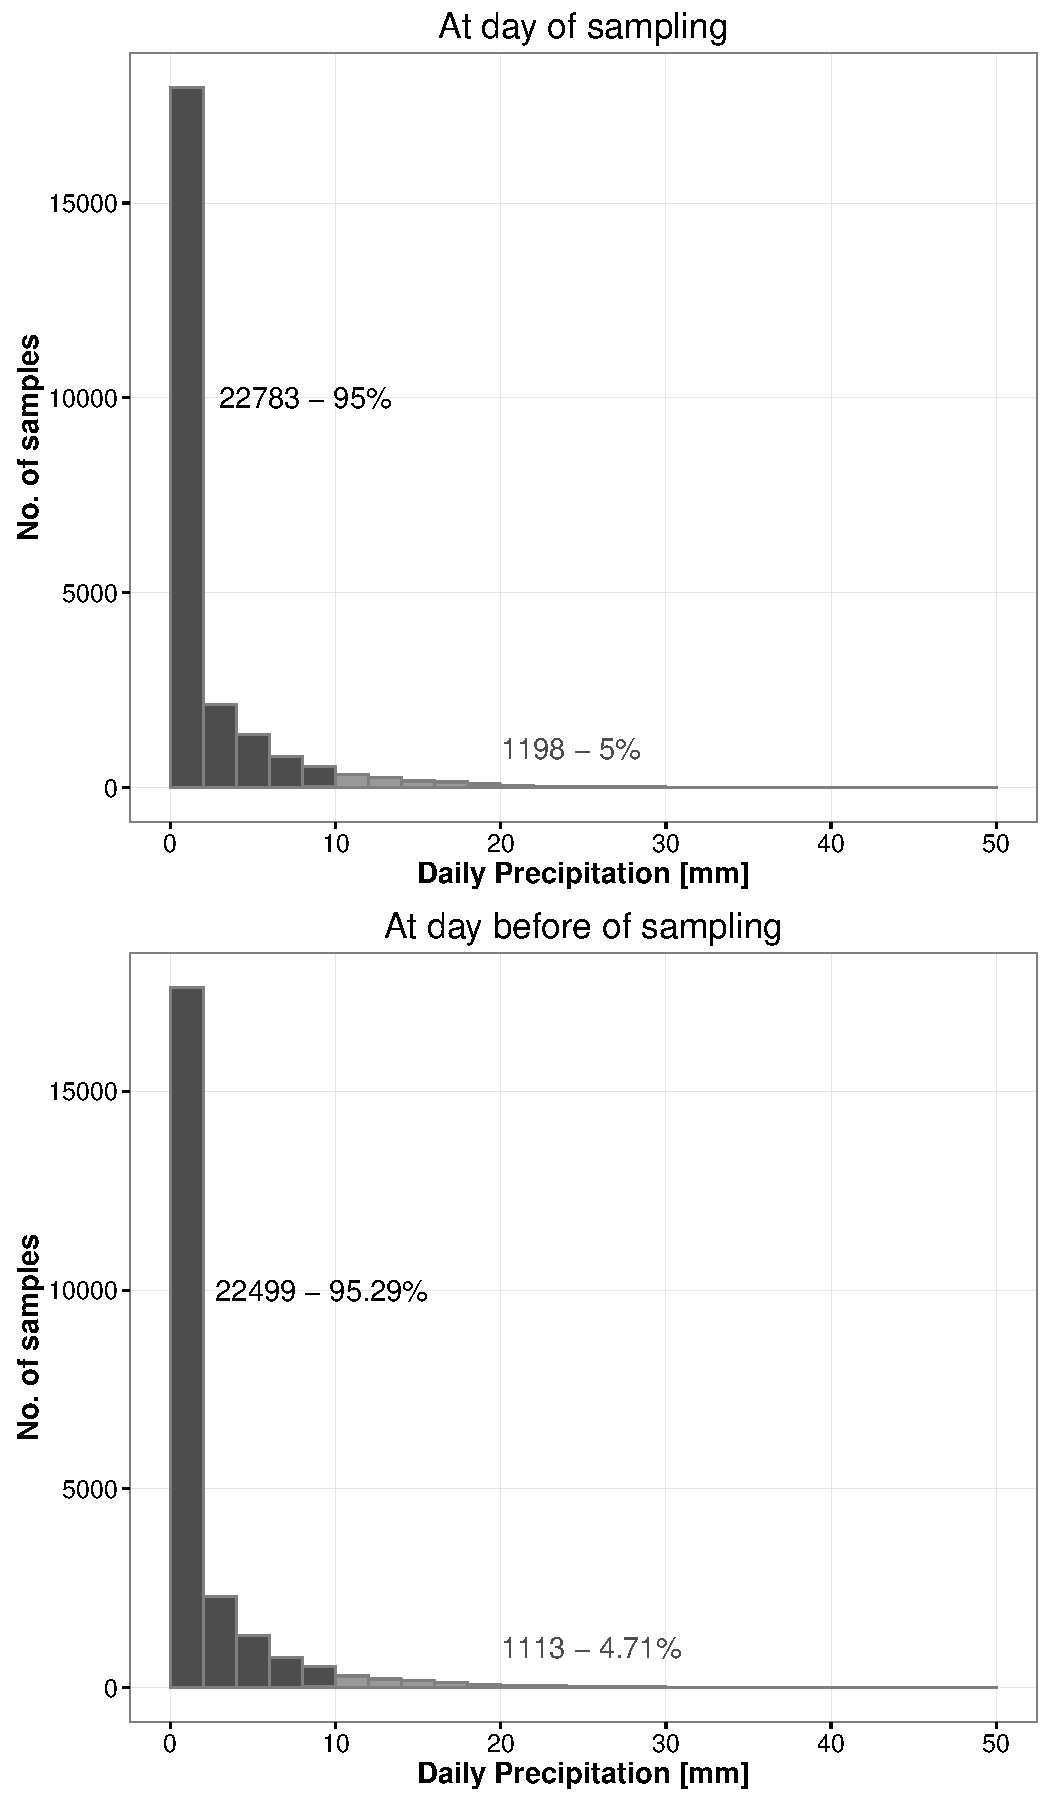
\includegraphics[width = 0.75\textwidth]{precip}
\caption{Distribution of precipitation at sampling occasions. top: at sampling date. bottom: at day before sampling.}
\label{fig:precip}
\end{figure}



\bibliographystyle{apalike}      % basic style, author-year citations
\bibliography{references}

\end{document}
